\startchapter{Graphs of StreamIt Benchmarks}
\label{chap:stream-graphs}

This appendix contains stream graphs for the StreamIt benchmark suite
(detailed in Table~\ref{tab:lang-benchmarks}).  As described in
Table~\ref{tab:lang-benchmarks-params}, many of the graphs are
parameterized, and we often assign small values to the parameters in
order to facilitate visualization and comprehension of the graph.
Graphs with different sizes, shapes, and work distributions can be
obtained by varying the parameters.

The stream graphs reflect the structure of the original input program,
prior to any transformations by the compiler.  In practice, the
compiler canonicalizes each graph by removing redundant
synchronization points, flattening nested pipelines, and collapsing
data-parallel splitjoins.  With the exception of GMTI and
MPEG2~\footnote{The stream graphs for GMTI and MPEG2 are canonicalized
  by the compiler, in order to reduce their size and improve the
  visualization.}, this canonicalization is disabled to illustrate the
programmer's original intent.

In the stream graphs, each filter is annotated with the following
information:
\begin{itemize}
\item The filter name.

\item The number of items\footnote{Some items may contain multiple
  values.  For example, if a data channel carries items of array type,
  then the graphs illustrate the number of arrays pushed and popped
  per execution.} pushed and popped per execution of the filter.
\item The estimated work (number of cycles) per execution of the filter.
\item Peeking filters are annotated with the number of items peeked (but not popped) per exection.
\item Stateful filters are annotated as such.
\end{itemize}

Filters are also colored to indicate their approximate amount of work
relative to other filters in the same program.  The heaviest and
lightest filters in a program are assigned fixed colors, and
intermediate filters are colored on a linear scale between the two:

\begin{center}
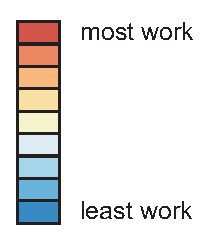
\psfig{file=color-scale.eps, height=1in}
\end{center}

\noindent Work estimates are gathered statically and may differ by 2x 
or more from actual runtime values.  Work estimates are not available
in some programs due to dynamic rates or Java subroutines.

%%%%%%%%%%%%%%%%%%%%%%%%%%%%%%%%%%%%%%%%%%%%%%%%%%%%%%%%%%%%%%%%%%%%%%%%

% some captions seem to need custom vspace
\newcommand{\tallgraphcustom}[3]{
\clearpage
\begin{figure}[t!]
\vspace{-12pt}
\centering
\psfig{file=apps/#1.eps,height=\textheight}
\vspace{#3}
\caption{Stream graph for #2.\protect\label{fig:#1-graph}}
\vspace{-12pt}
\end{figure}}

% default vspace
\newcommand{\tallgraph}[2]{\tallgraphcustom{#1}{#2}{-12pt}}

\newcommand{\widegraph}[2]{
\clearpage
\begin{figure}[t!]
\vspace{-12pt}
\hspace{-0.025\textwidth}\psfig{file=apps/#1.eps,width=1.05\textwidth}
\vspace{-12pt}
\caption{Stream graph for #2.\protect\label{fig:#1-graph}}
\vspace{-12pt}
\end{figure}}

\newcommand{\smallgraph}[2]{
\clearpage
\begin{figure}[t!]
\vspace{-12pt}
\centering
\psfig{file=apps/#1.eps,scale=0.7}
\vspace{-12pt}
\caption{Stream graph for #2.\protect\label{fig:#1-graph}}
\vspace{-12pt}
\end{figure}}

\tallgraphcustom{3GPP}{3GPP}{-24pt}
\tallgraph{802.11a}{802.11a}
\widegraph{Audiobeam}{Audiobeam}
\widegraph{Autocor}{Autocor}
\smallgraph{BitonicSort-(coarse)}{BitonicSort (coarse)}
\tallgraph{BitonicSort-(fine-iterative)}{BitonicSort (fine, iterative)}
\tallgraph{BitonicSort-(fine-recursive)}{BitonicSort (fine, recursive)}
\tallgraph{BubbleSort}{BubbleSort}
\widegraph{ChannelVocoder}{ChannelVocoder}
\tallgraph{Cholesky}{Cholesky}
\widegraph{ComparisonCounting}{ComparisonCounting}
\tallgraph{CRC}{CRC}
\tallgraph{DCT-(float)}{DCT (float)}
\tallgraph{DCT2D-(NxM-float)}{DCT2D (NxM, float)}
\widegraph{DCT2D-(NxN-int-reference)}{DCT2D (NxN, int, reference)}
\tallgraph{DES}{DES}
\tallgraph{DToA}{DToA}
\tallgraph{FAT}{FAT}
\tallgraph{FFT-(coarse-default)}{FFT (coarse, default)}
\widegraph{FFT-(fine-1)}{FFT (fine 1)}
\widegraph{FFT-(fine-2)}{FFT (fine 2)}
\tallgraph{FFT-(medium)}{FFT (medium)}
\tallgraph{FHR-(feedback-loop)}{FHR (feedback loop)}
\tallgraph{FHR-(teleport-messaging)}{FHR (teleport messaging)}
\widegraph{FMRadio}{FMRadio}
\smallgraph{Fib}{Fib}
\widegraph{FilterBank}{FilterBank}
\tallgraph{GMTI}{GMTI}
\widegraph{GP-particle-system}{GP - particle-system}
\widegraph{GP-phong-shading}{GP - phong-shading}
\widegraph{GP-reference-version}{GP - reference-version}
\widegraph{GP-shadow-volumes}{GP - shadow-volumes}
\widegraph{GSM}{GSM}
\tallgraph{H264-subset}{H264 subset}
\widegraph{HDTV}{HDTV}
\tallgraph{IDCT-(float)}{IDCT (float)}
\tallgraph{IDCT2D-(NxM-float)}{IDCT2D (NxM-float)}
\widegraph{IDCT2D-(NxN-int-reference)}{IDCT2D (NxN, int, reference)}
\smallgraph{IDCT2D-(8x8-int-coarse)}{IDCT2D (8x8, int, coarse)}
\widegraph{IDCT2D-(8x8-int-fine)}{IDCT2D (8x8, int, fine)}
\smallgraph{InsertionSort}{InsertionSort}
\widegraph{JPEG-decoder}{JPEG decoder}
\widegraph{JPEG-transcoder}{JPEG transcoder}
\tallgraph{Lattice}{Lattice}
\widegraph{MP3}{MP3}
\tallgraph{MPD}{MPD}
\tallgraph{MPEG2-decoder}{MPEG2 decoder}
\widegraph{MPEG2-encoder}{MPEG2 encoder}
\widegraph{MatrixMult-(coarse)}{MatrixMult (coarse)}
\widegraph{MatrixMult-(fine)}{MatrixMult (fine)}
\widegraph{MergeSort}{MergeSort}
\widegraph{Mosaic}{Mosaic}
\widegraph{OFDM}{OFDM}
\tallgraph{Oversampler}{Oversampler}
\widegraph{Radar-(coarse)}{Radar (coarse)}
\widegraph{Radar-(fine)}{Radar (fine)}
\tallgraph{RadixSort}{RadixSort}
\smallgraph{RateConvert}{RateConvert}
\smallgraph{Raytracer1}{Raytracer1}
\smallgraph{RayTracer2}{RayTracer2}
\tallgraph{SAR}{SAR}
\tallgraph{SampleTrellis}{SampleTrellis}
\tallgraph{Serpent}{Serpent}
\tallgraph{TDE}{TDE}
\widegraph{TargetDetect}{TargetDetect}
\smallgraph{VectAdd}{VectAdd}
\widegraph{Vocoder}{Vocoder}
